\section{Large Hadron Collider}
\label{ch:lhc}

This chapter describes the Large Hadron Collider 
(LHC)\nomenclature{LHC}{Large hadron collider} \cite{lhc-jinst}.
The LHC is a two-ring superconducting synchrotron, built and operated by the 
European Organization for Nuclear Research
(CERN)\nomenclature{CERN}{European organization for nuclear research}.
The LHC's main purpose is to accelerate two beams of protons in opposite directions
up to a nominal beam energy of 7~\TeV~and to collide them with an instantaneous 
luminosity\footnote{Instantaneous luminosity ($\mathcal{L}$) is defined  as the ratio
between the production rate in Hz for given physics process in a collider and the 
production cross section for that process.  Instantaneous luminosity depends only on beam parameters,
and it is expressed in units of $\text{cm}^{-2}\text{s}^{-1}$.  It is discussed in further detail
in Section \ref{sec:lhc-parameters}.  }
of up to $10^{34}$~$\text{cm}^{-2}\text{s}^{-1}$.
The LHC is also capable of colliding beams of lead ions ($^{208}_{82}\text{Pb}^{82+}$)
with a beam energy of up to 2.76~\TeV~per nucleon and an instantaneous luminosity
of up to $10^{27}$~$\text{cm}^{-2}\text{s}^{-1}$.  The remainder of this
chapter will discuss the LHC as it pertains to accelerating and colliding protons.
Section \ref{sec:lhc-structure} of this chapter describes the various components of the LHC 
and its injector complex, while Section \ref{sec:lhc-parameters} of this chapter
lists various parameters associated with LHC operations.

\subsection{LHC structure}
\label{sec:lhc-structure}

The LHC lies in a 26.7 km long tunnel about 100~m beneath
the suburbs of Geneva, Switzerland, as shown in Figure \ref{fig:lhc-map}.
The tunnel was dug between 1984 and 1989 and was
originally used for the Large Electron-Positron Collider
(LEP)\nomenclature{LEP}{Large electron-positron collider}.
\begin{figure}
  \centering
  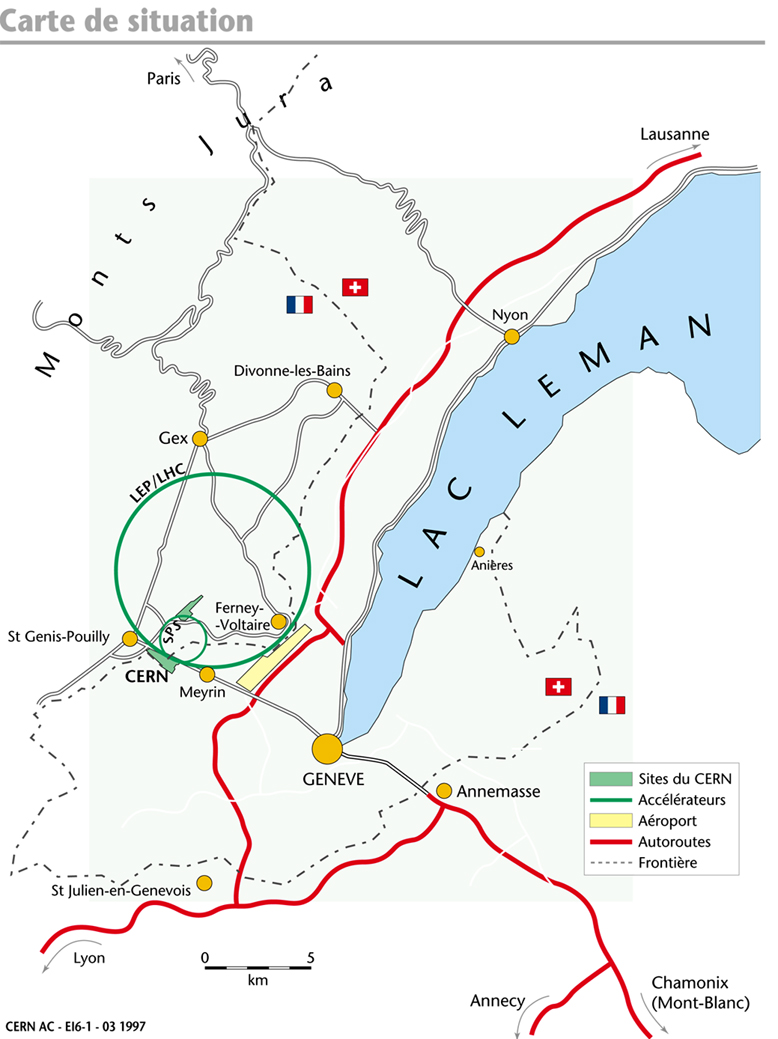
\includegraphics[width=1.0\textwidth]{tex/lhc/fig/lhc-map.jpg}
  \caption{Map of CERN, the LHC, the SPS, and the surrounding area \cite{lhc-map}.}
  \label{fig:lhc-map}
\end{figure}
Both the LHC and its tunnel are roughly circular, consisting of 
eight 2.45 km long arcs and eight 545 m long straight sections
called ``insertions'' that connect the arcs.

Each of the LHC's eight arcs contains 154 superconducting dipole magnets (1232 in total) 
designed to steer two proton beams in opposite directions around the LHC.
The dipole magnets contain two separate bores, each containing one of the proton
rings.  Each dipole magnet is 14.3 m long and weighs 35 tons.
The dipoles produce a field of up to 8.3 T using a current of 11,850 A, and
their superconductivity is maintained using liquid helium at 1.9 K. 
A cross section of an LHC dipole magnet is shown in Figure \ref{fig:lhc-dipole}.
\begin{figure}
  \centering
  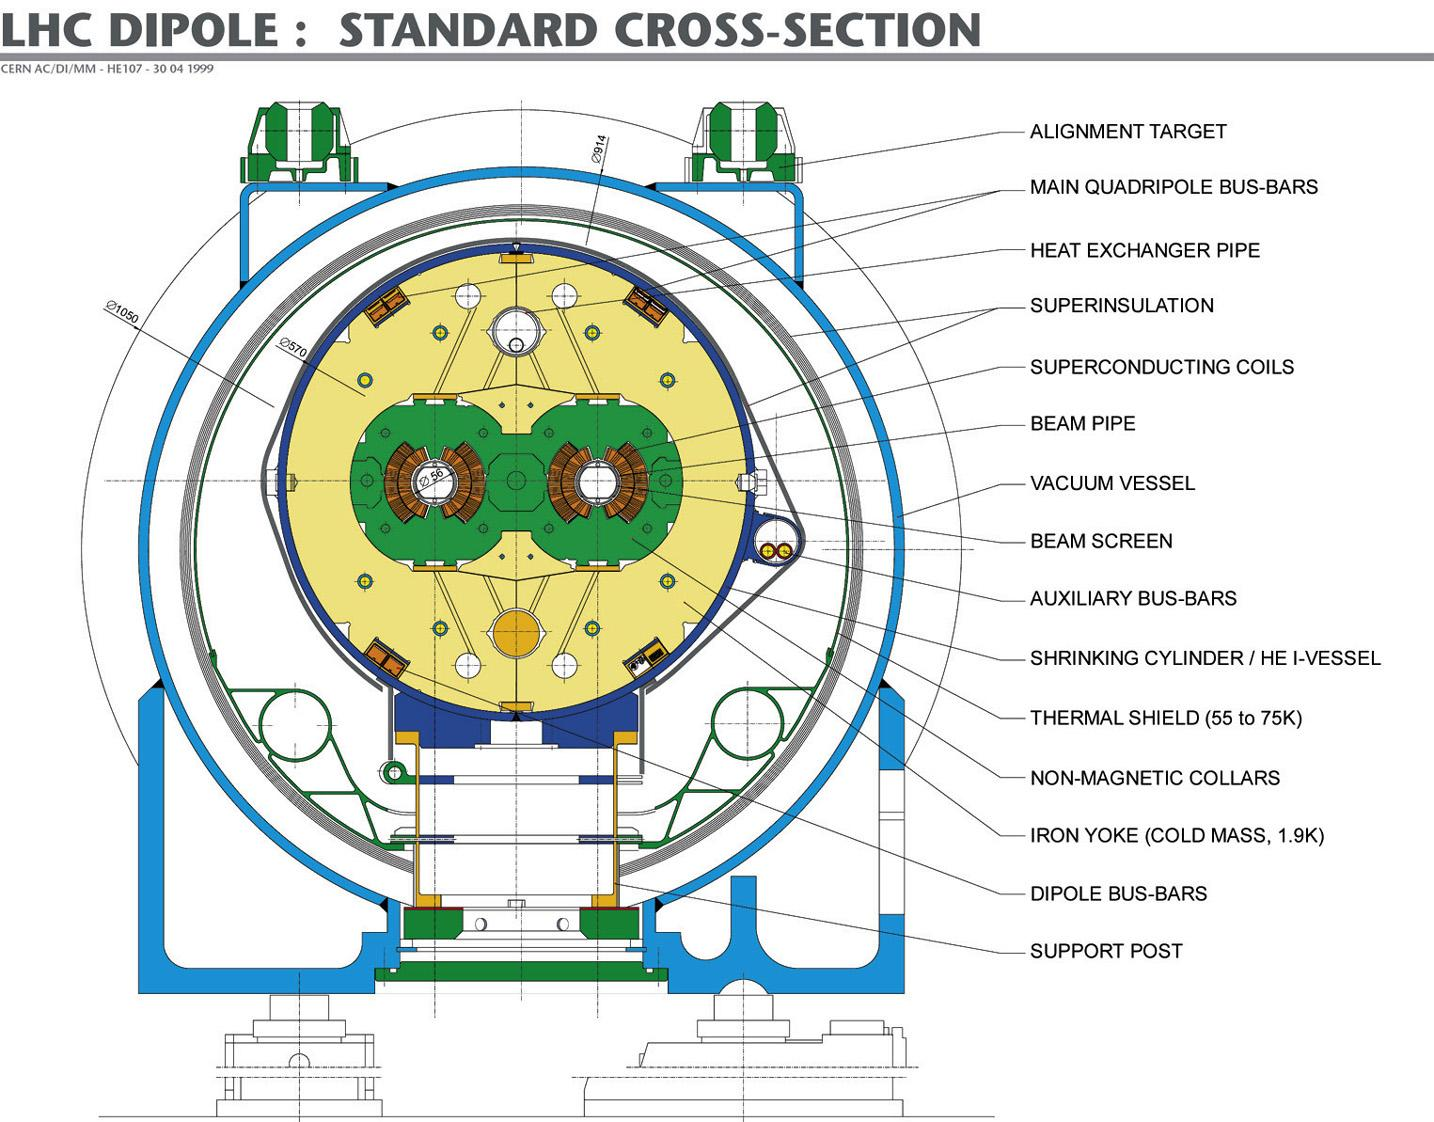
\includegraphics[width=0.6\textwidth]{tex/lhc/fig/lhc-dipole.jpg}
  \caption{Cross section of one of the 1232 LHC dipole magnets \cite{lhc-jinst}.}
  \label{fig:lhc-dipole}
\end{figure}

The contents of the LHC's eight insertions vary.  
The location of each insertion is described as a Point, and each
insertion-Point pair is given a number from 1 to 8.
The insertions at Points 1, 2, 5, and 8 serve as interaction points,
where proton beams cross from one magnet bore to the other and collide within
a 130~m long common section.
These four interaction points are the sites of four particle detectors,
each designed to record the results of high energy particle collisions.
Two of these detectors, 
``A Toroidal LHC ApparatuS'' (ATLAS, Point 1) 
\cite{atlas-jinst}
\nomenclature{ATLAS}{A toroidal LHC apparatus}
and the ``Compact Muon Solenoid'' (CMS, Point 5) 
\cite{cms-jinst}
\nomenclature{CMS}{Compact muon solenoid}
are general purpose detectors designed to study high luminosity collisions.
The ``Large Hadron Collider beauty'' detector (LHCb, Point 8) 
\cite{lhcb-jinst}
\nomenclature{LHCb}{Large hadron collider beauty}
is designed to study the physics of bottom quarks.
``A Large Ion Collider Experiment'' (ALICE, Point 2) 
\cite{alice-jinst}
\nomenclature{ALICE}{A large ion collider experiment}
is a detector designed to study heavy ion collisions.
The insertions at Points 3 and 7 contain beam collimation systems.
The insertion at Point 4 contains two radio frequency (RF)
\nomenclature{RF}{Radio frequency} cavity systems, designed
to accelerate the proton beams to higher energies.
Each RF cavity system contains eight RF cavities, and each RF cavity delivers
2 megavolts at 400 MHz. 
The insertion at Point 6 contains systems for dumping the beam from the LHC.  Each beam
has its own dumping system.
A section of the LHC beginning in the middle of one arc and ending in the middle
of an adjacent arc (and thereby containing one entire insertion) is called an octant.
Octants are labeled with the same number as the interaction point they contain.  
A schematic of the various octants can be seen in Figure \ref{fig:lhc-machine}.
\begin{figure}
  \centering
  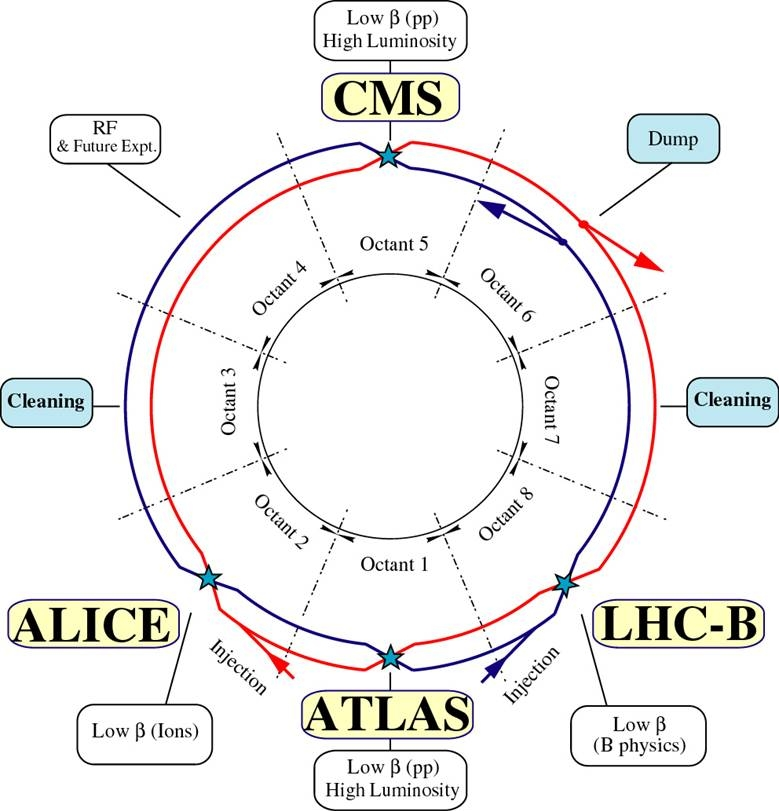
\includegraphics[width=0.6\textwidth]{tex/lhc/fig/lhc-machine.jpg}
  \caption{Schematic of the LHC including the octants, the role
    of the insertion within each octant, and the major experiments \cite{lhc-jinst}}
  \label{fig:lhc-machine}
\end{figure}

The accelerator complex at CERN serves as the injector for the LHC.
The complex is responsible for extracting protons from a bottle
of hydrogen gas, accelerating them in stages to 450 GeV, and injecting them into the LHC.
Protons are extracted from hydrogen gas by means of a duoplasmatron and 
injected into a linear accelerator (Linac2) where they are accelerated to 50 MeV.
The protons are then passed through a chain of three synchrotron accelerators.
First, the protons are transfered to the Proton Synchrotron Booster (PSB),
\nomenclature{PSB}{Proton synchrotron booster} where they are accelerated to 
1.4 GeV.  Next, the protons are transfered to the Proton Synchrotron (PS),
\nomenclature{PS}{Proton synchrotron} where they arranged in bunches and accelerated
to 25 GeV.  Finally, the protons are transfered to the Super Proton Synchrotron (SPS),
\nomenclature{SPS}{Super proton synchrotron} where they are accelerated to 450 GeV
before being injected into the LHC. A schematic of the CERN accelerator complex is 
shown in Figure \ref{fig:lhc-complex}.
\begin{figure}
  \centering
  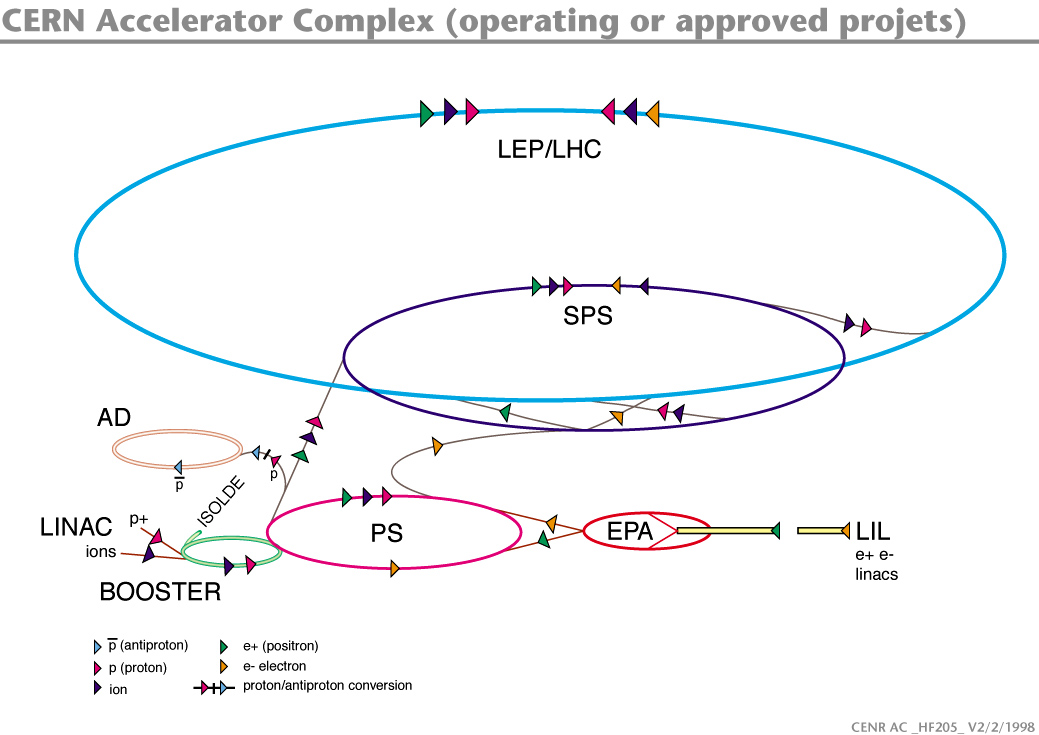
\includegraphics[width=0.6\textwidth]{tex/lhc/fig/lhc-injector-complex.jpg}
  \caption{ Schematic of the CERN accelerator complex \cite{lhc-complex}}
  \label{fig:lhc-complex}
\end{figure}

The arrangement of the beam into bunches as described in the previous 
paragraph is an important concept.  Protons are injected into the LHC 
in bunches spaced 25 ns apart.  Collisions within the LHC primarily
take place when bunches cross path at the interaction points.  These
25 ns ``bunch crossings'' form a window in time during which the detectors
described above record as much information about a $pp$ interaction as they can
before the next bunch crossing arrives.

\subsection{LHC operating parameters}
\label{sec:lhc-parameters}

The LHC was designed to search for rare physics processes (i.e.
processes with a small production cross section).  A critical 
element involved in searching for these processes is an estimate
of the rate (in Hz) with which they will be produced.  The ratio
between the production rate of a physics process in a collider and the
production cross section of that process is known as ``instantaneous luminosity'', $\mathcal{L}$, 
and it is measured in units of $\text{cm}^{-2}\text{s}^{-1}$.  
``Integrated luminosity'', \Lint, refers to an integral of instantanenous luminosity
over a period of time, and it is expressed in units of $\text{cm}^{-2}$.
The relationship between instantaneous luminosity, $\mathcal{L}$, 
the production cross section for a given physics process, $\sigma_{\text{event}}$, 
and the number of events produced, $N_{\text{event}}$, is given by Equation \ref{eqn:general-lumi}:
\begin{equation}
  N_{\text{event}} = \int\sigma_{\text{event}} \mathcal{L} dt
  \label{eqn:general-lumi}
\end{equation}
Luminosity depends only on beam parameters.  In the case of the LHC,
instantaneous luminosity may be calculated using Equation \ref{eqn:lhc-lumi}:
\begin{equation}
  \mathcal{L} = \frac{N_b^2n_bf_{\text{rev}} \gamma_r }{4\pi\varepsilon_n\beta^{*}} F
  \label{eqn:lhc-lumi}
\end{equation}
where 
$N_b$ is the number of protons in a bunch,
$n_b$ is the number of bunches in a beam,
$f_{\text{rev}}$ is the revolution frequency,
$\gamma_r$ is the relativistic gamma factor,
$\varepsilon_n$ is the transverse beam emmitence,
$\beta^{*}$ is the value of the beta function at the interaction point (IP),
\nomenclature{IP}{Interaction point}
and $F$ is the geometric luminosity reduction factor due to the crossing
angle between the two beams at the IP.  $F$ may be calculated using
Equation \ref{eqn:lhc-lumi-factor}:
\begin{equation}
  F = \left(1 + \frac{\theta_c\sigma_z}{2\sigma^{*}}\right)^{-1/2}
  \label{eqn:lhc-lumi-factor}
\end{equation}
where 
$\theta_c$ is the crossing angle at the IP,
$\sigma^*$ is the RMS of the transverse beam size at the IP, and
$\sigma_z$ is the RMS of the bunch length.  This relationship 
assumes round beam profiles and equal parameters for both beams.
The nominal values for each of these parameters at the LHC may be found in
Table \ref{tab:lhc-parameters}.

\begin{table}
  \centering
  \begin{tabular}{c|c|c|c}
    \multicolumn{2}{c|}{Parameter} & Unit & Nominal value \\ 
    \hline\hline
    $N_b$ & number of particles per bunch & & $1.15 \cdot 10^{11}$ \\
    $n_b$ & number of bunches per beam & & 2808 \\ 
    $f_\text{rev}$ & revolution frequency & kHz & 11.246 \\
    $\gamma_r$ & relativistic $\gamma$ factor & & 7461 \\
    $\varepsilon_n$  & transverse beam emittance & $\mu$m &  3.75 \\
    $\beta^{*}$ & beta function at the IP & m & 0.55 \\
    $F$ & geometric $\mathcal{L}$ reduction factor & & 0.836 \\
    $\theta_c$ & crossing action at IP & $\mu$rad & 285 \\ 
    $\sigma_z$ & RMS bunch length & cm & 7.55 \\
    $\sigma^*$ & RMS beam size at the IP & $\mu$m & 16.7 \\ 
    \hline
    $\mathcal{L}$ & Instantaneous luminosity & $\text{cm}^{-2}\text{s}^{-1}$ & $10^{34}$ \\
  \end{tabular}
  \caption{Nominal LHC beam parameters
    contributing to the luminosity, $\mathcal{L}$,
    as defined in Equation \ref{eqn:lhc-lumi}.
    \cite{lhc-jinst}}
  \label{tab:lhc-parameters}
\end{table}

The nominal conditions described in Table \ref{tab:lhc-parameters}
differ somewhat from the conditions under which the LHC 
operated during its first three years of running.
The peak instantaneous luminosity achieved during stable $pp$ collisions as
of December 2012 was $0.767 \cdot 10^{34}\text{cm}^{-2}\text{s}^{-1}$ (77\% of nominal).
This value was achieved with 1368 colliding bunches (49\% of nominal).
In addition, the LHC has only run with a maximum beam energy of 4 TeV (57\% of nominal).
The maximum instantaneous luminosity and beam energy for each year between 2010 and 2012 is shown
in Table \ref{tab:lhc-lumi-values}.
The integrated luminosity that the LHC delivered to Point 5 for the years 2010 through 2012 is
shown as a function of time in Figure \ref{fig:lumi}.

\begin{table}
  \centering
  \begin{tabular}{c|c|c}
    &  Beam energy & Maximum instantaneous $\mathcal{L}$ \\
    Year &(TeV) & $(10^{34}\text{cm}^{-2}\text{s}^{-1})$ \\
    \hline\hline
    2010 & 3.5 & 0.021 \\
    2011 & 3.5 & 0.354 \\ 
    2012 & 4.0 & 0.767 \\
    \hline
    Nominal & 7.0 & 1.0 \\
  \end{tabular}
  \caption{The LHC beam energy and maximum
    instantaneous luminosity at Point 5 (CMS) for the years 2010-2012, as compared with nominal design values \cite{cms-lumi}}
  \label{tab:lhc-lumi-values}
\end{table}

\begin{figure}
  \centering
  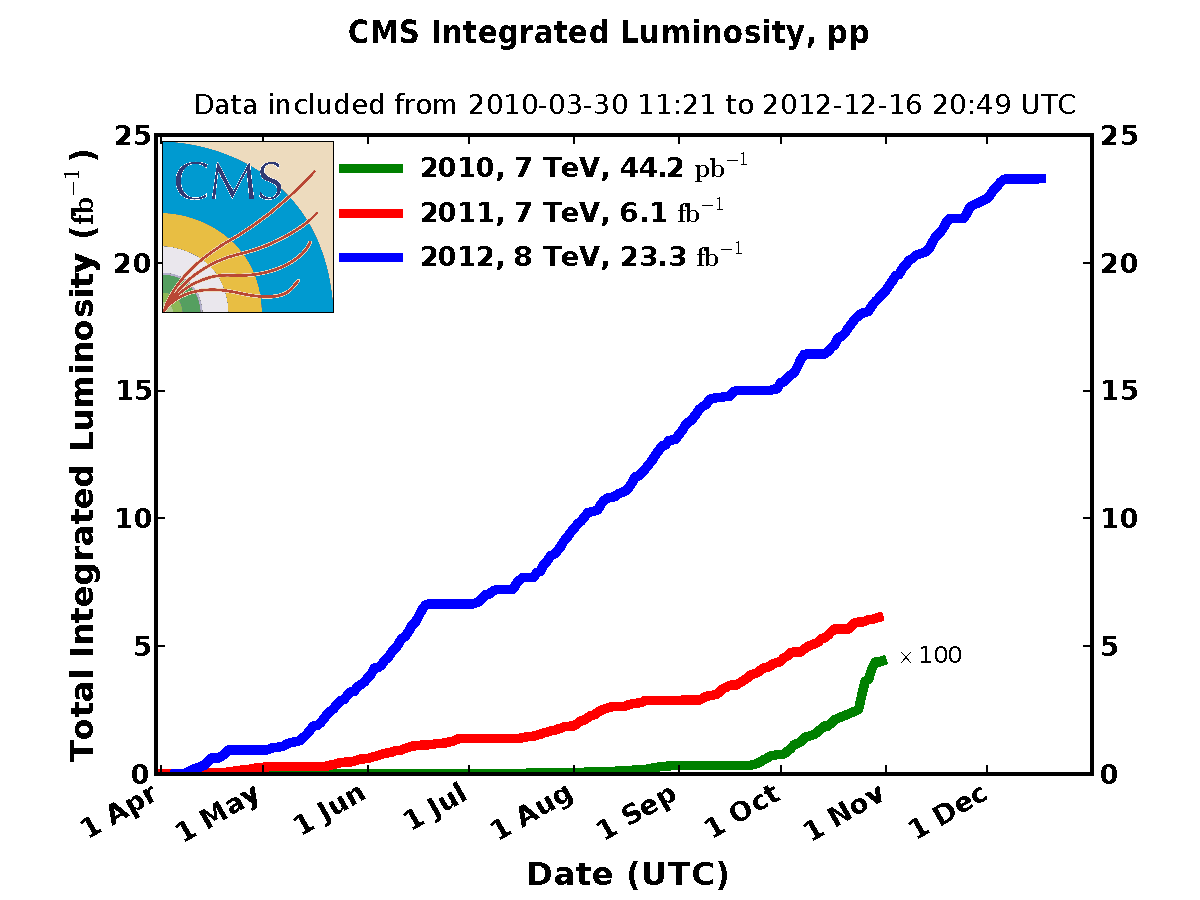
\includegraphics[width=0.6\textwidth]{tex/lhc/fig/int_lumi_cms.pdf}
  \caption{Total integrated luminosity delivered by the LHC to Point 5 (CMS) as a function of time, for the years 2010-2012 \cite{cms-lumi}}
  \label{fig:lumi}
\end{figure}
